\section[C. 星之所在]{\myboxiii{      \BF{\TT{C}}} 星之所在}

\textit{运行时间限制}   1 second

\textit{内存使用限制} 1 Gigabyte

\textit{读入文件} \qquad 标准输入

\textit{输出文件} \qquad 标准输出


\begin{quote}
	\textit{Star farming 是我国古代的伟大发现。}
\end{quote}

\subsection{题目描述}

Ph\textbf{eo}nix 来到了外太空，这里有 $n$ 个星系，它们的编号分别为 $1$, $2$, $\ldots$, $n$, 这些星系通过 $n - 1$ 条双向虫洞通道相互连接，每个星系都可以经由这些虫洞通道相互抵达。

每个星系包含一些恒星，$i$ 号星系拥有的恒星数量为 $s_i$.

Pheonix 将要进行 $q$ 次星系之间穿越虫洞的旅行，在一次旅行中 Pheonix 不会重复前往去过的星系。


Pheonix 对天文了解有限，但 Pheonix 的数学观察力很敏锐，对于每次旅行他想要询问小 T 这样的问题：

\begin{itemize}
	\item 将从星系 $x$ 到星系 $y$ 的虫洞旅行中会经过的星系（包括起点和终点）的恒星数量放进一个可重集合 $S$ 中，也即 $S = \{s_i : i\ \text{在} \ x \ \text{到}\  y\ \text{的路径上}\}$.
	\item $S$ 中是否存在元素满足其出现次数严格大于 $\frac{|S|}{k}$? 其中 $k$ 是 Pheonix 在每次提问中指定的一个整数。若有则求出有哪些。
\end{itemize}

请帮助小 T 回答这些问题。

\subsection{输入格式}

第一行输入一个整数 $T$ ($ 1 \le T \le 10^5$), 表示测试数据的数量。

每组测试数据第一行输入两个整数 $n$ 和 $q$ ($2 \le n \le 10^5, 1 \le q \le 10^5$), 表示星系数量和 Pheonix 的旅行次数。

随后一行输入 $n$ 个整数 $s_1$, $s_2$, $\ldots$, $s_n$ ($1 \le s_i \le n$), 分别表示这些星系所拥有的恒星数量。

随后 $n - 1$ 行每行输入两个整数 $u$ 和 $v$ ($1 \le u, v \le n, u \ne v$), 表示存在一条连接 $u$ 和 $v$ 的虫洞通道。

随后 $q$ 行每行输入 $3$ 个整数 $x$, $y$, $k$ ($1 \le x, y \le n, 2 \le k \le n, x \ne y$), 表示 Pheonix 的一次旅行的起点和终点，以及提问的参数。

保证所有测试数据的 $\sum n, \sum q, \sum k \le 3 \times 10^5$, 保证每组测试数据中的虫洞通道满足每个星系都可以经由这些虫洞通道相互抵达。

\subsection{输出格式}

对于每组测试数据输出 $q$ 行，第 $i$ 行输出第 $i$ 次提问的答案：
\begin{itemize}
	\item 若存在 $S$ 中元素满足其出现次数严格大于 $\frac{|S|}{k}$, 则按照恒星数量大小从小到大输出（而非按照出现次数）恒星数量。
	\item 否则输出一个整数 $-1$.
\end{itemize}

\subsection{样例 1}

\begin{minipage}{\linewidth}
	\begin{minipage}[t]{0.49\linewidth}
		\begin{lstlisting}[title=\texttt{standard input}]
2
6 4
1 2 2 1 2 3
1 2
2 3
2 4
4 5
5 6
3 6 2
1 4 3
1 6 2
1 5 3
7 5
1 2 1 3 2 2 4
1 2
1 3
2 4
2 5
3 6
6 7
4 5 2
4 7 3
5 6 4
3 1 2
7 5 2
\end{lstlisting}
	\end{minipage}
	\begin{minipage}[t]{0.49\linewidth}
		\begin{lstlisting}[title=\texttt{standard output}]
2
1
-1
1 2
2
-1
1 2
1
-1
\end{lstlisting}
	\end{minipage}
\end{minipage}


\subsection{样例 1 解释}


\begin{figure}[htbp]
   \centering
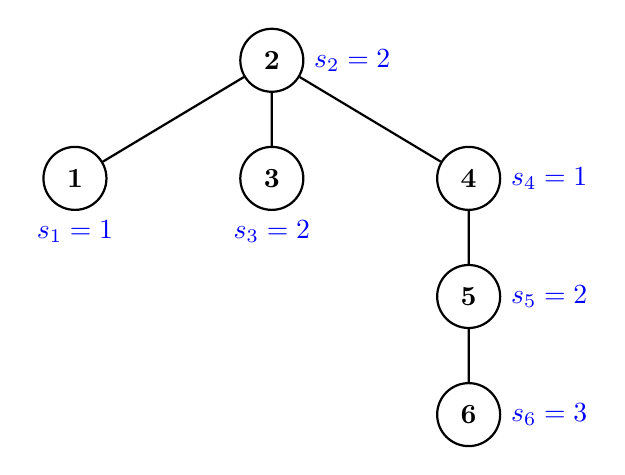
\begin{tikzpicture}[
    level 1/.style={sibling distance=2.5cm},
    level 2/.style={sibling distance=2cm},
    level distance=1.5cm,
    galaxy/.style={circle, draw=black, thick, minimum size=0.8cm, font=\bfseries},
    edge from parent/.style={draw=black, thick}
]

% 根节点：星系 2
\node[galaxy, label={[text=blue]right:$s_2=2$}] {2}
    % 星系 2 的三个子节点：1, 3, 4
    child { node[galaxy, label={[text=blue]below:$s_1=1$}] {1} }
    child { node[galaxy, label={[text=blue]below:$s_3=2$}] {3} }
    child { node[galaxy, label={[text=blue]right:$s_4=1$}] {4}
        % 星系 4 的子节点：5
        child { node[galaxy, label={[text=blue]right:$s_5=2$}] {5}
            % 星系 5 的子节点：6
            child { node[galaxy, label={[text=blue]right:$s_6=3$}] {6} }
        }
    };

\end{tikzpicture}
\end{figure}

上面的图展示了第 1 组测试数据的虫洞链接情况和恒星数量。

第 1 组询问从 $3$ 号星系到 $6$ 号星系，参数为 $2$, 经过的星系编号为 $3 \rightarrow 2 \rightarrow 4 \rightarrow 5 \rightarrow 6$, 恒星数量分别为 $S = \{2, 2, 1, 2, 3\}$, 满足出现次数严格大于阈值 $\frac{|S|}{k} = 2.5$ 的恒星数量为 $2$.





